% !TEX program = xelatex
% 光遗传学与视网膜退化性疾病的视觉功能恢复 · 四材料十六问（39 分，选择题强化版）
% 编译：xelatex -interaction=nonstopmode -halt-on-error 本文件（跑两遍）
\documentclass[UTF8,a4paper,11pt]{ctexart}

\usepackage{geometry}
\geometry{left=1.9cm,right=1.9cm,top=2.3cm,bottom=2.3cm}
\usepackage{graphicx}
\usepackage{amsmath,amssymb}
\usepackage{booktabs}
\usepackage{longtable}
\usepackage{array}
\usepackage{enumitem}
\usepackage{xcolor}
\usepackage{caption}
\usepackage{float}
\usepackage{titlesec}
\usepackage{fancyhdr}
\usepackage[hidelinks]{hyperref}

\graphicspath{{../命题图/}{../../Resources/Downloads/原图-光遗传学视觉恢复/}}

\definecolor{deepblue}{HTML}{1F4E79}
\definecolor{deepred}{HTML}{C00000}
\definecolor{deepgreen}{HTML}{2E7D32}

\captionsetup{font=small,labelfont=bf,skip=4pt}
\titleformat{\section}{\Large\bfseries\color{deepblue}}{\thesection}{0.6em}{}
\titleformat{\subsection}{\normalsize\bfseries\color{deepblue}}{\thesubsection}{0.6em}{}
\pagestyle{fancy}
\fancyhf{}
\fancyhead[L]{\small 光遗传学与视觉功能恢复 · 四材料十六问（39 分）}
\fancyhead[R]{\small\thepage}

\newcommand{\pt}[1]{\textbf{（#1分）}}
\newcommand{\lv}[1]{{\small\color{deepgreen}［#1］}}
\newcommand{\key}[1]{\textbf{\color{deepred}#1}}
\newcommand{\tian}[1]{\underline{\hspace{#1}}}
\newcommand{\choice}[1]{\par\smallskip\noindent #1\par}

\title{\bfseries 光遗传学与视网膜退化性疾病的视觉功能恢复\\[5pt]
\large 四材料 · 十六问综合题（39 分 · 选择题强化版）}
\author{}\date{2026-10-06}

\begin{document}
\maketitle
\thispagestyle{fancy}

\begin{center}
\fbox{\parbox{0.95\textwidth}{\small
\textbf{阅读提示}：科研事实取自 Pan et al. 2014、Lu et al. 2016、Lu et al. 2018 三篇开放获取论文。
专业名词均在材料或表注中给出\textbf{做题所需的全部解释}，不需事先记忆；标"\key{命题简化}"的数据，其数值为命题需要而设定，趋势依原论文改写。
本题共 16 小问、39 分，其中\textbf{单选 3、多选 4、编号选填 1、编号排序 1，客观题共 9 问（占 17 分）}。
}}
\end{center}

\section*{命题说明}
\addcontentsline{toc}{section}{命题说明}

\begin{table}[H]
\centering\small
\begin{tabular}{@{}llcccc@{}}
\toprule
\textbf{题号} & \textbf{题型} & \textbf{考查落点} & \textbf{难度} & \textbf{分值} & \textbf{部分} \\
\midrule
Q1 & 单选 & 视网膜细胞分工 & 基础 & 2 & Ⅰ \\
Q2 & 多选 & RP 与治疗的性质辨析 & 基础 & 2 & Ⅰ \\
Q3 & 简答 & 信号通路中断的后果 & 基础 & 3 & Ⅰ \\
Q4 & 简答 & 基因表达→蛋白功能→细胞功能 & 中等 & 3 & Ⅰ \\
Q5 & 编号排序 & 据表比较光敏性 & 基础 & 2 & Ⅰ \\
Q6 & 多选 & 光敏性与时间响应的关系 & 中等 & 2 & Ⅰ \\
Q7 & 简答 & 多指标权衡（优势与局限） & 拔高 & 3 & Ⅰ \\
Q8 & 编号选填+简答 & 据表选择方案并说明理由 & 中等 & 3 & Ⅱ \\
Q9 & 多选 & 载体与调控元件的功能 & 中等 & 2 & Ⅱ \\
Q10 & 简答 & 表达量 ≠ 功能（证据层级） & 拔高 & 3 & Ⅱ \\
Q11 & 单选 & 据表判断恢复效果最好者 & 中等 & 2 & Ⅱ \\
Q12 & 单选 & 双因素读表（空间频率与光强） & 中等 & 2 & Ⅱ \\
Q13 & 简答 & 实验变量分析 & 中等 & 3 & Ⅱ \\
Q14 & 多选 & 对照与评价指标 & 拔高 & 2 & Ⅱ \\
Q15 & 简答 & 对照的必要性与多指标评价 & 拔高 & 2 & Ⅱ \\
Q16 & 简答·开放 & 优化方案与依据 & 拔高 & 3 & Ⅱ \\
\midrule
\multicolumn{4}{r}{\textbf{合计}} & \textbf{39} & \\
\bottomrule
\end{tabular}
\end{table}

\noindent\textbf{分值结构}：客观题（单选／多选／编号选填／编号排序）9 问共 17 分，占 44\%；简答与分析 7 问共 22 分。
\textbf{难度分层}：基础 9 分（Q1、Q2、Q3、Q5）；中等 15 分（Q4、Q6、Q8、Q9、Q11、Q12、Q13）；拔高 15 分（Q7、Q10、Q14、Q15、Q16）。

\noindent\textbf{使用建议}：本材料题组可整体使用（39 分），也可\textbf{按"部分Ⅰ／Ⅱ"拆为两道大题}——第Ⅰ部分（材料一、二，15 分）、第Ⅱ部分（材料三、四与综合，24 分）。

\section{材料一\quad 视觉损伤与治疗思路}
\addcontentsline{toc}{section}{材料一：视觉损伤与治疗思路}

视网膜像一台"光信号转换器"，把进入眼内的光变成神经信号送往大脑。视网膜中的\textbf{感光细胞}（视杆细胞与视锥细胞）负责感受光并把光信号转变为电信号；信号随后经\textbf{双极细胞}传到\textbf{神经节细胞}，后者的轴突汇聚成视神经，把信号送往大脑皮层视觉中枢，最终形成视觉（图1）。

视网膜色素变性（RP）是一类由基因突变引起的遗传性眼病。患者的\textbf{感光细胞逐渐死亡}，而内层的双极细胞与神经节细胞大多仍然存活。由于信号的"第一站"缺失，患者即使眼球结构和视神经通路完好，视觉功能仍会逐渐下降。

研究者尝试用\textbf{光遗传学}方法恢复视觉：把一种来自单细胞藻类的\textbf{光敏蛋白基因（ChR2 基因）}导入残存的视网膜细胞。ChR2 蛋白能在细胞膜上形成\textbf{受光控制的离子通道}——受到蓝光照射时通道开放，阳离子内流，细胞因此产生电位变化。

\begin{figure}[H]
\centering
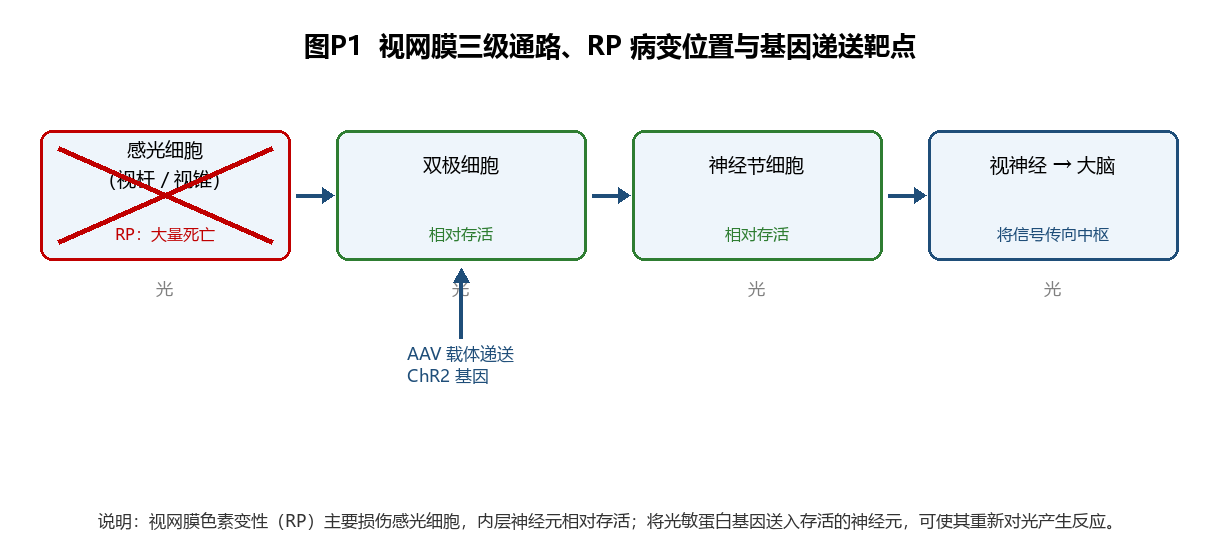
\includegraphics[width=0.68\textwidth]{P1_视网膜三级通路与病变.png}
\caption{图1\quad 视网膜三级细胞通路、RP 的主要受损环节与治疗靶点（简化示意图）}
\end{figure}

\subsection*{问题}

\begin{enumerate}[leftmargin=2.2em,itemsep=5pt]
\item \lv{单选} \pt{2} 在\textbf{正常}的视网膜中，直接把光信号转变为电信号的细胞是（\quad）\\
\choice{A. 感光细胞 \quad B. 双极细胞 \quad C. 神经节细胞 \quad D. 视神经}

\item \lv{多选} \pt{2} 结合材料，关于 RP 与光遗传学治疗，下列说法合理的有（\quad）（错选得 0 分）\\
\choice{A. RP 患者感光细胞大量死亡，而双极细胞与神经节细胞大多存活\\
B. 把 ChR2 基因导入残存神经细胞后，这些细胞在蓝光照射下可产生电位变化\\
C. 光遗传学治疗从根本上修复了患者致病的基因，因此可治愈 RP\\
D. 治疗后视觉信号仍需经神经节细胞传至大脑皮层视觉中枢才能形成视觉}

\item \lv{基础} \pt{3} 根据材料与图1，分析感光细胞退化为什么会引起视觉功能下降。

\item \lv{中等} \pt{3} 研究者把 ChR2 基因导入残存的视网膜神经细胞后，这些细胞便能在蓝光照射下产生反应。结合材料说明这一过程发生的可能机制（要求体现"基因表达 → 蛋白质功能 → 细胞功能"的链条）。
\end{enumerate}

\section{材料二\quad ChR2 突变体}
\addcontentsline{toc}{section}{材料二：ChR2 突变体}

天然 ChR2 有一个明显不足：需要在较强的光下才能被有效激活。研究者通过改变 ChR2 基因中特定位置的碱基序列，获得了多种\textbf{突变体}，并测定了它们的性能（表1）。

\begin{table}[H]
\centering\small
\caption*{\textbf{表1}\quad ChR2 及其突变体的性能比较（\key{命题简化}数据，相对值）}
\begin{tabular}{@{}lcccc@{}}
\toprule
\textbf{变体} & \textbf{阈值光强} & \textbf{弱光下光电流} & \textbf{通道关闭时间（响应时间）} & \textbf{高频闪烁下的响应能力} \\
\midrule
wt-ChR2（天然型） & 10 & 1.0 & 最短 & 强 \\
ChR2-L132C & 4 & 2.4 & 较长 & 中 \\
ChR2-L132C/T159C & 3 & 3.1 & 长 & 弱 \\
ChR2-L132C/T159S & 2 & 4.0 & 最长 & 很弱 \\
\bottomrule
\end{tabular}

\smallskip
\parbox{0.94\textwidth}{\footnotesize 注：\textbf{阈值光强}指能使细胞产生可检测光电流所需的最低光强，数值越小表示在越弱的光下即可被激活；\textbf{光电流}是通道开放时离子流动形成的电流，光电流越大表示对光越敏感；\textbf{通道关闭时间}指光照停止后通道关闭、细胞恢复静息状态所需的时间，时间越长表示细胞"恢复"越慢，对随时间快速变化的光信号（如闪烁、运动）的跟随能力越弱。数据为命题简化，趋势依据 Pan et al., 2014 改写。}
\end{table}

\subsection*{问题}

\begin{enumerate}[leftmargin=2.2em,itemsep=5pt,start=5]
\item \lv{编号排序} \pt{2} 根据表1，把四种变体按\textbf{光敏性由高到低}排序（填变体名称）：\\
\tian{2.5cm} $>$ \tian{2.5cm} $>$ \tian{2.5cm} $>$ \tian{2.5cm}

\item \lv{多选} \pt{2} 据表1，下列说法正确的有（\quad）（错选得 0 分）\\
\choice{A. ChR2-L132C/T159S 的阈值光强最低，在弱光下最容易被激活\\
B. 光敏性越高的变体，其通道关闭时间越短\\
C. 在高频闪烁刺激下响应能力最强的变体是 wt-ChR2\\
D. 就现有数据看，光敏性与时间响应特性可以同时达到最优}

\item \lv{拔高} \pt{3} 某突变体的光敏性显著提高，但其时间响应特性有所下降。请结合表1 分析该突变体用于视觉恢复时的\textbf{优势}与\textbf{局限}，并说明这是否意味着"光敏性最高就等于视觉恢复效果最好"。
\end{enumerate}

\section{材料三\quad AAV 递送与目标细胞靶向表达}
\addcontentsline{toc}{section}{材料三：AAV 递送与靶向表达}

把基因送入细胞需要"载体"。研究者使用\textbf{腺相关病毒（AAV）}作为载体：它能把携带的基因送入细胞，且本身引起的免疫反应较弱。但仅有载体还不够——基因在哪些细胞里表达、表达多少，取决于与目的基因连接在一起的\textbf{调控元件}（启动子与增强子）：启动子决定基因在什么条件下"开启"，增强子能加强这种表达。

研究者设计了三种构建方案（方案中目的基因与载体其余部分相同，只有调控元件不同），并检测了小鼠视网膜中的表达情况（表2）。图2 是把 ChR2 与红色荧光蛋白 mCherry 融合后，与能特异标记双极细胞的 PKC 抗体共同标记的结果：若红色荧光（表示基因表达）与绿色荧光（表示双极细胞）大量重叠，说明目的基因主要表达在双极细胞中。

\begin{table}[H]
\centering\small
\caption*{\textbf{表2}\quad 三种构建方案的表达情况比较（\key{命题简化}数据，相对水平）}
\begin{tabular}{@{}llccc@{}}
\toprule
\textbf{方案} & \textbf{调控元件} & \textbf{ChR2 总表达量} & \textbf{双极细胞中表达比例} & \textbf{非目标细胞中表达情况} \\
\midrule
甲 & 200 bp 增强子 + SV40 启动子 & 中 & 中 & 较明显 \\
乙 & 内源 mGluR6 启动子 + 200 bp 增强子 & 较高 & 高 & 很少 \\
丙 & 内源 mGluR6 启动子 + 内含子增强子 & 高 & 很高 & 极少 \\
\bottomrule
\end{tabular}

\smallskip
\parbox{0.94\textwidth}{\footnotesize 注：\textbf{mGluR6 调控元件}是与双极细胞中某基因表达相关的调控序列，本研究用它来提高目的基因在双极细胞中的表达；数据为命题简化，趋势依据 Lu et al., 2016 结果改写。}
\end{table}

\begin{figure}[H]
\centering
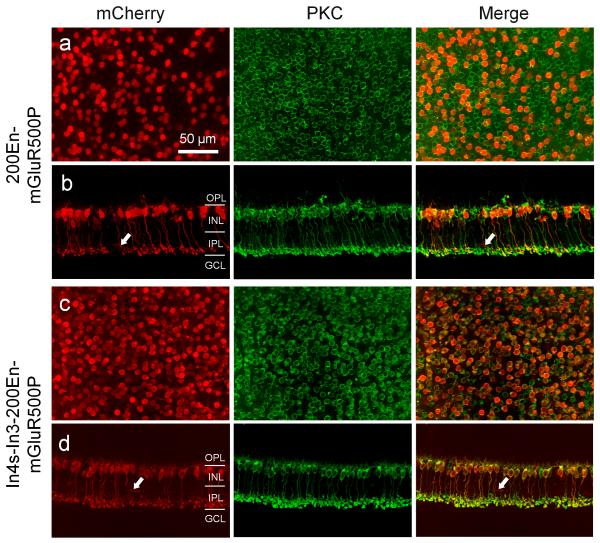
\includegraphics[width=0.72\textwidth]{Lu2016-Fig04.jpg}
\caption{图2\quad 论文原图（Lu et al., 2016, Fig.~4）：目的基因表达产物（红）与双极细胞标记物（绿）的共标结果}
\end{figure}

\subsection*{问题}

\begin{enumerate}[leftmargin=2.2em,itemsep=5pt,start=8]
\item \lv{编号选填+简答} \pt{3}
\begin{enumerate}[label=(\arabic*),leftmargin=1.4em,itemsep=2pt]
\item 根据表2，更适合实现"目的基因主要在双极细胞中表达"的方案是\tian{0.9cm}（填"甲""乙"或"丙"）（1 分）
\item 说明你作出上述判断的理由（2 分）。
\end{enumerate}

\item \lv{多选} \pt{2} 关于 AAV 载体与调控元件，下列说法正确的有（\quad）（错选得 0 分）\\
\choice{A. AAV 的作用是把目的基因送入细胞，属于基因工程中的载体\\
B. 启动子与增强子决定目的基因在哪些细胞中表达以及表达量的高低\\
C. 只要提高 ChR2 的总表达量，就一定能提高视觉恢复效果\\
D. 目的基因在非目标细胞中大量表达，可能干扰视网膜原有的信号处理}

\item \lv{拔高} \pt{3} 有同学认为："只要让视网膜细胞表达出尽可能多的 ChR2，视觉恢复效果就一定最好。"请结合材料二、材料三说明这一观点为什么不全面。
\end{enumerate}

\section{材料四\quad 用 OMR 评价视觉功能是否恢复}
\addcontentsline{toc}{section}{材料四：用 OMR 评价视觉功能是否恢复}

细胞是否"对光有反应"，不等于动物是否"看得见"。为评价视觉功能是否真正恢复，研究者使用\textbf{视动反应（OMR）}：把小鼠放在能显示移动条纹的装置中，若小鼠能看清条纹，其头部会随条纹运动方向转动；条纹越密集（\textbf{空间频率}越高），看清越困难，需要的光也越强。

研究者把三种 ChR2 变体分别导入三组同种失明小鼠，并设置一组\textbf{未经相同基因治疗处理}的小鼠作对照，测定了各组出现 OMR 所需的最低光强（表3）。

\begin{table}[H]
\centering\small
\caption*{\textbf{表3}\quad 各组小鼠出现 OMR 所需的最低光强（\key{命题简化}数据，相对值；"—"表示未出现 OMR）}
\begin{tabular}{@{}lccc@{}}
\toprule
\textbf{组别} & \textbf{低空间频率} & \textbf{中空间频率} & \textbf{高空间频率} \\
\midrule
未经基因治疗的对照组 & — & — & — \\
wt-ChR2 组 & 20 & $>$40 & — \\
ChR2-L132C 组 & 12 & 22 & $>$50 \\
ChR2-L132C/T159C 组 & 8 & 15 & 30 \\
ChR2-L132C/T159S 组 & 5 & 9 & 18 \\
\bottomrule
\end{tabular}
\end{table}

\subsection*{问题}

\begin{enumerate}[leftmargin=2.2em,itemsep=5pt,start=11]
\item \lv{单选} \pt{2} 在相同条件下，视觉功能恢复效果最好的一组是（\quad）\\
\choice{A. wt-ChR2 组 \quad B. ChR2-L132C 组\\
C. ChR2-L132C/T159C 组 \quad D. ChR2-L132C/T159S 组}

\item \lv{单选} \pt{2} 据表3，随空间频率（条纹密集程度）升高，各组出现 OMR 所需的最低光强（\quad）\\
\choice{A. 逐渐升高 \quad B. 逐渐降低 \quad C. 保持不变 \quad D. 先降低后升高}

\item \lv{中等} \pt{3} 若研究目的是"比较两种 ChR2 突变体对视觉恢复的影响"，请写出该实验的\textbf{自变量}、\textbf{因变量}，以及至少两个需要控制相同的变量。\tian{0.48\textwidth}

\item \lv{多选} \pt{2} 关于该实验，下列说法正确的有（\quad）（错选得 0 分）\\
\choice{A. 设置未经基因治疗的对照组，可用于排除其他因素引起 OMR 的可能\\
B. 各组小鼠的遗传背景、载体注射量与测定时间应保持一致\\
C. 视网膜中 ChR2 表达量越高，说明视觉恢复效果一定越好\\
D. OMR 是否出现属于行为学指标，比单纯检测蛋白表达更能反映视觉功能}

\item \lv{拔高} \pt{2} 请回答下列两个问题（各 1 分）：
\begin{enumerate}[label=(\arabic*),leftmargin=1.4em,itemsep=2pt]
\item 为什么必须设置"未经相同基因治疗处理"的对照组？
\item 除 OMR 外，还可以用什么指标评价视觉功能是否恢复？为什么评价疗效不宜只看一项指标？
\end{enumerate}
\end{enumerate}

\section{综合题}
\addcontentsline{toc}{section}{综合题}

\begin{enumerate}[leftmargin=2.2em,itemsep=5pt,start=16]
\item \lv{拔高·开放} \pt{3} 研究者希望进一步优化治疗方案。请根据上述全部材料，从"\textbf{ChR2 本身}、\textbf{目标细胞表达}、\textbf{刺激条件}、\textbf{功能评价}"中选择一个或多个角度，提出一种合理的优化思路，并说明依据。
\end{enumerate}

\clearpage
\section*{参考答案与评分细则}
\addcontentsline{toc}{section}{参考答案与评分细则}

\begin{longtable}{@{}p{0.9cm}p{9.5cm}p{4.3cm}@{}}
\toprule
\textbf{题} & \textbf{参考答案} & \textbf{评分点} \\
\midrule
\endhead
Q1 & \textbf{A}。感光细胞负责感受光并把光信号转变为电信号；双极细胞、神经节细胞是其后逐级传递信号的神经元。 & 选 A 得 2 分，其余 0 分。 \\
\addlinespace
Q2 & \textbf{ABD}。C 错：光遗传学并未修复致病基因，而是让残存细胞"获得"光响应能力，属于功能补偿，不是根治。 & 选 ABD 得 2 分；选 AB、AD、BD 得 1 分；含 C 或其他错选得 0 分。 \\
\addlinespace
Q3 & 感光细胞是视网膜形成视觉信号的\textbf{第一站}，其功能是把光信号转变为电信号；这些细胞退化死亡后，光信号无法被转换，位于其下游的双极细胞、神经节细胞虽存活却\textbf{得不到输入}，视网膜无法向大脑输出信号，故视觉功能下降（严重时失明）。 & 说出感光细胞的功能 1 分；指出信号在视网膜第一站中断 1 分；体现"下游细胞存活但无输入"1 分。仅答"因为细胞死了"不得分。 \\
\addlinespace
Q4 & 导入的 ChR2 基因在细胞内\textbf{转录、翻译}出 ChR2 蛋白；该蛋白\textbf{定位到细胞膜上}，形成能被光控制的离子通道；蓝光照射时通道开放、阳离子内流，使\textbf{膜电位发生改变}，细胞由此产生电信号（光响应）。 & 基因表达出蛋白 1 分；蛋白定位于膜上并形成受光调控的通道 1 分；光照→离子内流→膜电位改变→产生电信号 1 分。缺少"膜电位改变／产生电信号"扣 1 分。 \\
\addlinespace
Q5 & ChR2-L132C/T159S $>$ ChR2-L132C/T159C $>$ ChR2-L132C $>$ wt-ChR2 & 顺序完全正确得 2 分；顺序错误或漏项得 0 分。 \\
\addlinespace
Q6 & \textbf{AC}。B 错：表1 显示光敏性越高的变体，通道关闭时间越长；D 错：现有数据恰好体现"光敏性越高、时间响应越差"的权衡。 & 选 AC 得 2 分；选 A 或 C 得 1 分；含 B 或 D 得 0 分。 \\
\addlinespace
Q7 & \textbf{优势}：该突变体阈值光强最低、弱光下光电流最大，即在很弱的光下即可被激活，适合弱光环境（夜间、室内）使用。\textbf{局限}：其通道关闭时间最长，细胞恢复静息慢，对随时间快速变化的光信号（高频闪烁、运动）跟随能力最差，动态视觉信息可能难以分辨。\textbf{结论}：光敏性高只是"更容易被激活"，而视觉恢复还要求能分辨随时间变化的信息，故"光敏性最高"不等于"恢复效果最好"。 & 优势（弱光下易被激活）1 分；局限（响应变慢→动态分辨下降）1 分；得出"需多指标权衡、光敏性最高≠恢复最好"1 分。只答"它更敏感"不得分。 \\
\addlinespace
Q8 & (1) \textbf{丙}。(2) 丙方案在目标细胞（双极细胞）中的表达比例最高、在非目标细胞中的表达极少，说明其调控元件能使目的基因\textbf{主要限制在双极细胞中表达}，细胞特异性最好；同时其总表达量也最高，为产生足够的光响应提供了基础。 & (1) 填"丙"1 分。(2) 依据"目标细胞比例高"1 分；依据"非目标细胞表达少（特异性好）"或"总表达量高（为功能提供基础）"1 分。只答"丙最好"未给理由不得分。 \\
\addlinespace
Q9 & \textbf{ABD}。C 错：总表达量提高只说明产生了更多 ChR2 蛋白，若表达在非目标细胞中或蛋白功能（如响应速度）不合适，视觉恢复效果未必更好。 & 选 ABD 得 2 分；选 AB、AD、BD 得 1 分；含 C 得 0 分。 \\
\addlinespace
Q10 & 不全面。① 表达量只说明细胞里产生了多少 ChR2 蛋白，属于\textbf{蛋白水平}，是必要条件而非充分条件；② 材料三表明，若表达发生在\textbf{非目标细胞}中，既不能形成有效的视觉信号，还可能干扰视网膜原有的信号处理；③ 材料二表明，蛋白\textbf{功能是否合适}还取决于响应时间等指标——光敏性高但响应慢不利于分辨动态信息；④ 最终还必须看动物在\textbf{行为水平}（OMR）上是否出现功能改善。 & 指出"表达量是蛋白水平、必要但不充分"1 分；答出"须表达在正确的细胞"或"蛋白功能要合适"1 分；答出"须以行为学等功能性指标为准"1 分。 \\
\addlinespace
Q11 & \textbf{D}（ChR2-L132C/T159S 组）。该组在三种空间频率下出现 OMR 所需的最低光强都最小，说明在相同条件下其视觉功能恢复最好。 & 选 D 得 2 分；其余 0 分。 \\
\addlinespace
Q12 & \textbf{A}（逐渐升高）。条纹越密集越难分辨，需要更强的光才能引出 OMR。 & 选 A 得 2 分；其余 0 分。 \\
\addlinespace
Q13 & \textbf{自变量}：导入的 ChR2 突变体类型（并设未经相同基因治疗处理的对照组）。\textbf{因变量}：是否出现 OMR、出现 OMR 所需的最低光强。\textbf{控制变量}（答出两个）：小鼠的遗传背景与生理状态（同一失明模型）、注射的载体量与浓度、注射后至测定的时间、光刺激的波长与强度、条纹的空间频率等。 & 自变量 1 分（须体现"不同突变体"且含对照）；因变量 1 分；控制变量答出两个 1 分。 \\
\addlinespace
Q14 & \textbf{ABD}。C 错：表3 显示各组都能表达 ChR2，但出现 OMR 所需的最低光强明显不同，说明表达量不能代表视觉功能恢复程度。 & 选 ABD 得 2 分；选 AB、AD、BD 得 1 分；含 C 得 0 分。 \\
\addlinespace
Q15 & (1) 排除"失明小鼠本身、注射操作或光刺激"等也能引起 OMR 的可能，证明观察到的反应\textbf{确实来自导入的 ChR2}，使因果判断成立。(2) 还可以用\textbf{瞳孔对光收缩}等指标；因为不同指标反映视觉功能的不同方面（瞳孔反射反映对光的觉察能力，OMR 还涉及对移动图像的分辨与中枢整合），只用一项指标可能得出片面结论。 & (1) 排除其他因素、证明因果 1 分；(2) 举出合理指标 0.5 分，说明"需多指标／单一指标片面"0.5 分。 \\
\addlinespace
Q16 & 角度与依据（答出一个角度并说明依据即可）：\textbf{① ChR2 本身}——在保持较高光敏性的同时筛选响应更快的变体（依据 Q7／Q11：光敏性与响应时间存在权衡，响应快有利于分辨运动信息）。\textbf{② 目标细胞表达}——优化调控元件使表达更集中于双极细胞（依据 Q8／Q10：非目标细胞表达少可减少干扰、提高特异性）。\textbf{③ 刺激条件}——优化光刺激的波长、强度与频率，使之与所用变体匹配（依据 Q7／Q11：不同变体对不同光强、不同模式刺激的响应不同）。\textbf{④ 功能评价}——增加瞳孔对光反射、多空间频率下的 OMR 等指标（依据 Q12／Q15：功能评价应多层次）。 & 优化方向合理且能从前文推出 1 分；依据与方向匹配并引用具体材料或数据 1 分；表述完整、逻辑清楚 1 分。方向脱离材料（如"用干细胞替换视网膜"）不得分。 \\
\bottomrule
\end{longtable}

\section*{命题底线自检}
\addcontentsline{toc}{section}{命题底线自检}

\begin{longtable}{@{}p{0.6cm}p{6.0cm}p{8.2cm}@{}}
\toprule
\textbf{\#} & \textbf{底线要求} & \textbf{落实情况} \\
\midrule
\endhead
1 & 不要求学生背诵 ChR2、mGluR6、AAV 的专业定义 & 三者均以"材料给定的含义"出现；选择题选项只考查其\emph{功能角色}（通道蛋白、载体、调控序列），不考定义式记忆。 \\
\addlinespace
2 & 首次出现的专业事实必须给出必要解释 & 阈值光强、光电流、通道关闭时间、空间频率、OMR、启动子/增强子、共标均在材料或表注中解释。 \\
\addlinespace
3 & 不使用大学电生理学作为直接考点 & 未要求解释动作电位的离子机制或通道动力学；"响应时间"只作表中信息用于比较。 \\
\addlinespace
4 & 不要求记忆实验编号、载体编号、品系名称 & 全文无载体编号、血清型与小鼠品系名称。 \\
\addlinespace
5 & 专业数据经过高中化处理 & 表1—表3 均为相对值并标注"命题简化"，趋势依原文改写。 \\
\addlinespace
6 & 高难度来自多证据整合 & Q7（表1 两列指标权衡）、Q10（材料二＋三整合）、Q16（四段材料整合）难点均在证据整合与变量分析。 \\
\addlinespace
7 & 每个结论都有材料或高中知识支持 & 逐问核查：Q1—Q4（图1＋材料一）、Q5—Q7（表1）、Q8—Q10（表2）、Q11—Q15（表3）、Q16（前文全部）。 \\
\bottomrule
\end{longtable}

\section*{附录\quad 论文原图对照（课堂延伸用）}
\addcontentsline{toc}{section}{附录：论文原图对照}

\begin{figure}[H]
\centering
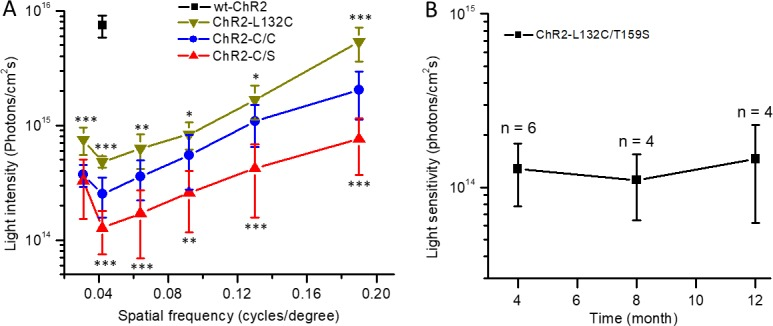
\includegraphics[width=0.78\textwidth]{Lu2018-Fig04.jpg}
\caption{图A\quad 论文原图（Lu et al., \textit{IOVS}, 2018, Fig.~4）：三种 ChR2 变体的 OMR 阈值光强—空间频率关系，与表3 趋势一致，供课堂延伸或按真实数据替换表3 时对照使用。}
\end{figure}

\noindent\small 全部 22 张论文原图与三篇文献（两篇全文 Markdown、一篇原版 PDF）存于 \texttt{00 - Personal/Resources/Downloads/}。

\end{document}
